\documentclass[]{beamer}
%\usetheme{boxes}
\beamertemplatenavigationsymbolsempty
\setbeamertemplate{footline}[page number]
% Set it for the internal PhD thesis defence to reduce number of slides
%\setbeamersize{text margin left=0.5em, text margin right=0.5em}

\usepackage[utf8]{inputenc}
%\usepackage[english, russian]{babel}
\usepackage{bm}
\usepackage{multirow}
\usepackage{ragged2e}
\usepackage{indentfirst}
\usepackage{multicol}
\usepackage{subfig}
\usepackage{amsmath,amssymb}
\usepackage{enumerate}
\usepackage{mathtools}
\usepackage{comment}
\usepackage[all]{xy}
\usepackage{tikz}
\usetikzlibrary{positioning,arrows}
\tikzstyle{name} = [parameters]
\definecolor{name}{rgb}{0.5,0.5,0.5}

%\usepackage{caption}
%\captionsetup{skip=0pt,belowskip=0pt}

%\newtheorem{theorem}{Theorem}
%\newtheorem{statement}{Statement}
%\newtheorem{definition}{Definition}

% colors
\definecolor{darkgreen}{rgb}{0.0, 0.2, 0.13}
\definecolor{darkcyan}{rgb}{0.0, 0.55, 0.55}
%\AtBeginEnvironment{figure}{\setcounter{subfigure}{0}}
%\captionsetup[subfloat]{labelformat=empty}

%--------------------------------------------------------------------------------------------

%\title{ Detecting Manual Alterations in Biological Image Data
%Using Contrastive Learning and Pairwise Image Comparison}
%\author{Georgii Nekhoroshkov}
%\institute[]{Moscow Institute of Physics and Technology}
%\date{March 27, 2025}

%---------------------------------------------------------------------------------------------
\begin{document}
%\begin{frame}
%\titlepage
%\end{frame}
%---------------------------------------------------------------------------------------------
%\section{Please do not use sectioning in the presentations}
%\begin{frame}{Identification of Fabricated Images}
%\begin{block}{The problem}
%Instances of fraud in biological science articles.
%\end{block}
%\begin{block}{The method}
%Developing a robust self-supervised pairwise image comparison model resistant to alterations.
%\end{block}
%\begin{block}{The solution}
%Building on ideas from Barlow Twins, the plan is as follows:
%\begin{enumerate}[1)]
%\item setup Barlow Twins model with pre-trained ResNet50 encoder,
%\item train model's projector on biological scans,
%\item train model's probability head.
%\end{enumerate}
%\end{block}
%\end{frame}
%---------------------------------------------------------------------------------------------
\begin{frame}{Identification of Fabricated Biological Images}
\begin{columns}
    \begin{column}{0.42\textwidth}
        \begin{block}{The problem}
        Detection of similar images despite modifications.
        \end{block}
    \end{column}
    \begin{column}{0.58\textwidth}
        \begin{block}{The solution}
        A Barlow Twins\footnotemark{}-based 
        model for pairwise image comparison.
        \end{block}
    \end{column}
\end{columns}

\medskip

\begin{columns}
    \begin{column}{0.42\textwidth}
        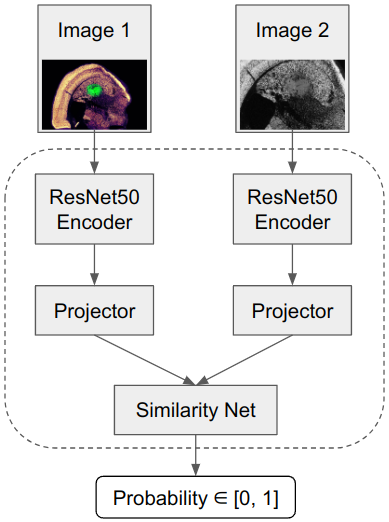
\includegraphics[width=0.86\textwidth]{model.png}
    \end{column}
    \begin{column}{0.58\textwidth}
        The model processes two images and outputs a value from [0, 1] --
        the likelihood that they are identical, up to modifications.
        
        \bigskip
        The method leverages a self-supervised learning approach.
    \end{column}
\end{columns}
\footnotetext{\textit{J. Zbontar et al.} Barlow Twins: Self-Supervised Learning via 
        Redundancy Reduction // ICML, 2021.}
\end{frame}
\end{document}
